\chapter[Gerenciamento dos Requisitos]{Gerenciamento dos Requisitos}

  \section{Atributos de requisitos}
  
    Os atributos de requisitos são as propriedades de um requisito. 
    Eles capturam informações importante que são utilizadas para uma melhor gerência dos requisitos e do projeto.
    
    Os atributos definidos para o projeto, visando um melhor gerenciamento dos requisitos, foram:
    
    \begin{figure}[!htbp]
      \centering
      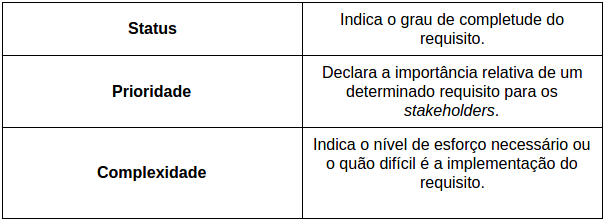
\includegraphics[scale=0.5]{editaveis/figuras/requirements_atributes}
      \caption[Atributos de requisitos do projeto] {Atributos de requisitos do projeto. \footnotemark}
      \label{requirements_atributes}
    \end{figure}
    
    A seguir são descritos os valores que podem ser assumidos por cada atributo:
    \textbf{Status:}
    \begin{itemize}
     \item \textbf{Completo/Realizado}: Indica que o requisito em questão foi realizado e implementado no sistema; 
     \item \textbf{Em Progresso}: Indica que o requisito em questão está em processo de implementação dentro do sistema;
     \item \textbf{Não Iniciado}: Indica que o requisito em questão foi submetido ao seu respectivo \textit{Backlog}, porém não foi iniciado o seu processo de implementação.
    \end{itemize}
    \textbf{Prioridade:}
    \begin{itemize}
     \item \textbf{Alta}: Indica que o requisito em questão é de suma importância para os \textit{stakeholders}, agregando grande valor aos usuários;
     \item \textbf{Média}: Indica que o requisito em questão possui relativa importância para os \textit{stakeholders}, podendo ser implementado quando for de interesse do cliente.
     \item \textbf{Baixa}: Indica que o requisito em questão possui pequena importância para os \textit{stakeholders}, representando uma funcionalidade opcional do sistema.
    \end{itemize}
    \textbf{Complexidade:}
    \begin{itemize}
     \item \textbf{Alta}: Indica que o requisito em questão possui alto nível de dificuldade, exigindo um grande nível de esforço para sua implementação;
     \item \textbf{Média}: Indica que o requisito em questão possui um relativo nível de dificuldade, exigindo um nível de esforço moderado para sua implementação;
     \item \textbf{Baixa}: Indica que o requisito em questão possui um baixo nível de dificuldade, exigindo um baixo nível de esforço para sua implementação.
    \end{itemize}
  
    Exemplo de matriz de atributos de requisitos:
    \begin{figure}[!htbp]
      \centering
      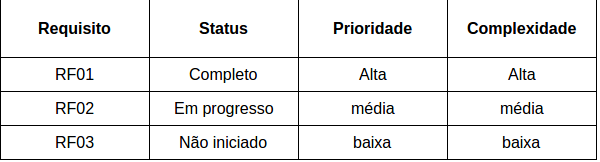
\includegraphics[scale=0.5]{editaveis/figuras/example_atributes}
      \caption[Exemplo do uso dos atributos de requisitos.] {Exemplo do uso dos atributos de requisitos.. \footnotemark}
      \label{example_atributes}
    \end{figure}
  
  
  \section{Estratégia de rastreabilidade}
  
    A rastreabilidade de requisitos é importante para prover relacionamentos entre requisitos, 
    arquitetura e implementação final do sistema de software, 
    possibilitando uma compreensão dos relacionamentos de dependência entre 
    requisitos e entre os requisitos e artefatos do sistema \cite{sayao05}.
  
    A rastreabilidade pode ser implementada através de um conjunto,
    dos chamados, elos de rastreabilidade entre requisitos inter-relacionados, 
    entre requisitos e suas fontes e entre requisitos e os componentes do sistema, 
    de acordo com Sayão e Leite (\citeyear{sayao05}).
  
    O elo é o principal recurso utilizado para manter e representar os relacionamentos da rastreabilidade. 
    Um elo é estabelecido entre um artefato origem e um artefato destino \cite{genvigir09}.
  
    \begin{figure}[!htbp]
      \centering
      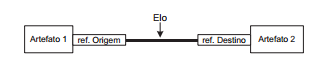
\includegraphics[scale=1]{editaveis/figuras/elo}
      \caption[Elementos básicos de um elo.] {Elementos básicos de um elo. \footnotemark}
      \label{elo}
    \end{figure}
    \footnotetext{Fonte: \cite{genvigir09}}
  
    De acordo com Genvigir (\citeyear{genvigir09}), 
    informações sobre a origem e o destino são suficientes para garantir a rastreabilidade para frente e para trás.
  
    Sayão e Leite (\citeyear{sayao05}), apresentam alguns tipos de elos de rastreabilidade 
    propostos em dois meta-modelos de rastreabilidade, 
    o Meta-modelo de Ramesh e Jarke e o de Toranzo.

    Ramesh e Jarke (\citeyear{ramesh01}), acreditam que os elos de rastreabilidade podem ser agrupados em duas categorias básicas:
    \begin{itemize}
      \item \textbf{Relacionados ao produto}: elos que descrevem propriedades e relacionamentos dos objetos. Sendo esses elos de satisfação e dependência.
      \item \textbf{Relacionados ao processo}: elos relacionados ao histórico de ações executadas no próprio processo. Sendo eles, elos de evolução  e elos de \textit{rationale} (indica as razões ou motivações para uma determinada ação).
    \end{itemize}

    Para a utilização na disciplina e no contexto desse relatório, 
    serão contemplados nesse trabalho, apenas, elos de rastreabilidade relacionados ao produto, 
    mais precisamente, os elos de dependência. Que segundo Ramesh e Jarke (\citeyear{ramesh01}), são definidos como:

    \begin{citacao}
      Elos de dependência têm por propósito apoiar o gerenciamento de dependências entre objetos, 
      freqüentemente impostas por restrições de recurso, de competência ou de compatibilidade, 
      sendo úteis para registrar a composição e hierarquia dos objetos e apoiar o gerenciamento do impacto das 
      alterações num objeto sobre os objetos que dele dependem. \cite{ramesh01}
    \end{citacao}
  
    Destacando que objetos são definidos por Ramesh e Jarke (\citeyear{ramesh01}) como sendo objetos conceituais 
    relacionados ao produto, como por exemplo requisitos, ou artefatos gerados no processo de desenvolvimento.

    Levando em consideração os  conceitos, definições e limitações supracitados, a estratégia de rastreabilidade de 
    requisitos para nosso contexto seguirá a hierarquia representada visualmente na figura a seguir:
  
    \begin{figure}[!htbp]
      \centering
      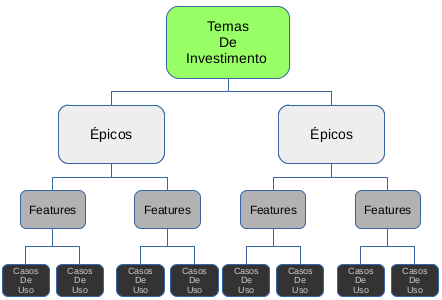
\includegraphics[scale=0.7]{editaveis/figuras/traceability}
      \caption[Diagrama - Estratégia de Rastreabilidade de Requisitos.] {Diagrama - Estratégia de Rastreabilidade de Requisitos. \footnotemark}
      \label{traceability}
    \end{figure}
 
    Os requisitos serão rastreados a partir do nível de portfólio, 
    através dos temas de investimento e épicos, e passarão pelos níveis de programa e time, 
    através das \textit{features} e casos de uso, respectivamente. Dessa forma, os requisitos serão rastreados para frente, 
    que segundo Davis (\citeyear{davis93}), é a capacidade de rastrear um requisito até seus refinamentos, 
    e para trás, que é a de rastrear um refinamento até sua origem.
  
    Para um maior controle e um melhor gerenciamento dos requisitos, 
    os mesmos serão identificados de acordo com a tabela a seguir:
  
    \begin{figure}[!htbp]
      \centering
      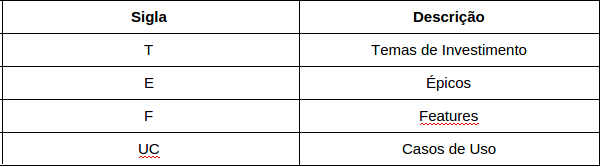
\includegraphics[scale=0.7]{editaveis/figuras/identificadores_requisitos}
      \caption[Identificadores dos requisitos]{Identificadores dos requisitos. \footnotemark}
      \label{identificadores_requisitos}
    \end{figure}
  
    Os requisitos serão nomeados a partir dos identificadores e, também, de acordo com sua fonte, ou seja, 
    o nome de um requisito será composto por:
  
    \begin{itemize}
      \item No caso de um \textbf{Tema de Investimento}: T (codigo tema investimento) Exemplo: T01.
      \item No caso de um \textbf{Épico}: T (codigo tema investimento) + E (codigo epico) Exemplo: T01E01.
      \item No caso de uma \textbf{Feature}: E (codigo epico) + F (codigo feature) Exemplo: E01F01.
      \item No caso de um \textbf{Caso de Uso}:  F (codigo feature) + UC (codigo caso uso) Exemplo: F01UC01.
    \end{itemize}

    Dessa forma, garantiremos a rastreabilidade para frente e para trás dos requisitos.
  
  \section{Ferramentas de gestão de requisitos}
    
    De acordo com Beatty (\citeyear{beatty13}), uma ferramenta de gerenciamento de requisitos deve oferecer
    suporte para armazenar requisitos especificados, armazenar artefatos relacionados (como modelos), permitir relações
    entre os requisitos, revisão e acompanhamento das mudanças nos requisitos e importar/exportar requisitos.
    
    Com isso em mente, foram escolhidas três ferramentas de RM (do inglês \textit{Requirements Management}) para análise de
    qual será a melhor para ser utilizada no projeto.  
    
    \subsection{Análise das ferramentas}
    
       
 As seguintes ferramentas foram analisadas:
 
 
  \begin{itemize}
   \item \textit{GatherSpace \footnotemark}
      
      \begin{itemize}
       \item
	  
	  O \textit{Gatherspace} é uma ferramenta paga, porém é possível acessar a versão \textit{trial} (versão de testes) por 30 dias.
	  A ferramenta fornece uma abordagem pragmática para organizações para capturar, gerenciar, documentar, modelar
	  o negócio, teste de sistemas de requisitos;
		  
       \item
	  
	  A ferramenta apresenta uma interface com o cliente interativa e intuitiva, afim de facilitar e simplificar o processo
	  de gerenciamento de requisitos. Os relatórios são diretos e claros afim de, novamente, tornar o processo mais simples.
	  Possibilita ao usuário ficar em contato com os outros stakeholders, pois o funciona em um ambiente \textit{web} e
	  possibilita participar em múltiplos projetos. Também fornece proteção contra perda de dados como documentos apagados,
	  sobrescritos ou modificados no ambiente online;
	  
       \item
	
	  De uma maneira geral, a ferramenta apresenta uma boa abrangência no que tange ao gerenciamento de requisitos, pois
	  contém funcionalidades para tratar dos pontos importantes para uma boa realização dessa atividade, desde definição
	  de atores e requisitos de negócio até modelos de caso de uso, relatório de rastreabilidade e relatório de busca
	  de \textit{bugs}.

      \end{itemize}
      \footnotetext{Fonte: http://www.gatherspace.com/}

   \item \textit{CASE Spec \footnotemark}
      
      \begin{itemize}
       \item 
	  
	  \textit{CASE Spec} fornece soluções para os problemas de gerenciamento de ciclo de vida no desenvolvimento de software e
	  sistemas, com uma abordagem simples que evita as longas curvas de aprendizagem. Fornece recursos na área de
	  especificação de requisitos e gerenciamento, análise de requisitos, colaboração, análise de rastreabilidade,
	  especificação de \textit{design} e documentação e testes. \textit{CASE Spec} não é uma ferramenta totalmente gratuita, mas é possível
	  utilizá-la por 30 dias sem custo, sendo necessário mandar um \textit{email} para a empresa e esta responderá com o
	  \textit{link} de \textit{download} do programa;
	  
       \item
	  
	  A ferramenta fornece integração com outras ferramentas como \textit{Microsoft Word, Excel, XML}, etc, que facilitam
	  a transição de um processo puramente focado em documentos para a ferramenta. Gera automaticamente relatórios detalhados e
	  especificação de documentos. Por utilizar uma abordagem baseada na \textit{Web}, a ferramenta permite maior integração
	  de todos os \textit{stakeholders} com o fluxo de trabalho relacionado ao projeto. As especificações do sistema podem ser
	  feitas tanto em histórias de usuários quanto em casos de uso e em lista de requisitos hierárquicos.

      \end{itemize}
      \footnotetext{Fonte: http://analysttool.com/}

    \item \textit{TestTrack \footnotemark}
      \footnotetext{Fonte: http://www.seapine.com/development-activity/requirements-management}
	
      \begin{itemize}

	\item 
	
	    O \textit{TestTrack} é uma ferramenta de gerenciamento do ciclo de vida da aplicação 
	    (do inglês \textit{Application Lifecycle Management}), sendo que possui como uma de suas funcionalidades
	    o gerenciamento dos requisitos. É paga, entretanto,possui um período de testes (\textit{trial}) de 30 dias,
	    o que torna possível utilizá-la de forma gratuita;
	    
	\item
	
	    Como uma de suas características destaca-se o fato de ser versátil, possuindo cliente nas versões para \textit{Windows, Mac} e
	    \textit{Linux}, além de um cliente \textit{online} (o que possibilita sua utilização independente do sistema operacional que está
	    sendo utilizado). Possui um bom foco na interação entre a equipe, também sendo possível verificar a rastreabilidade
	    dos requisitos de forma não complexa. Um dos problemas encontrados por essa ferramenta é a necessidade de um
	    servidor para a relação cliente-servidor;
	
	\item
	
	    O ponto que se destaca é a sua flexibilidade, sendo que é possível configurá-la para projetos que usam abordagens
	    que vão desde o cascata (tradicional) até ágeis.
	    
	  \begin{figure}[!htbp]
	    \centering
	    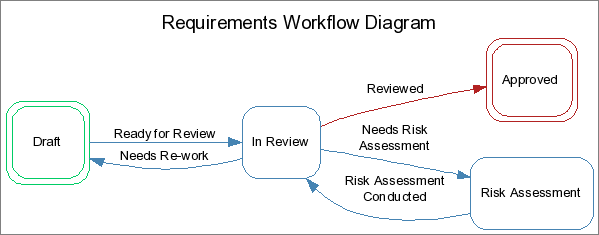
\includegraphics[scale=0.65]{editaveis/figuras/workflow_testtrack}
	    \caption[Exemplo de um diagrama de workflow de requisitos no TestTrack]
		{Diagrama de \textit{workflow} de requisitos no \textit{TestTrack}. \footnotemark}
	    \label{workflow_testtrack}
	  \end{figure}
	  \footnotetext{Disponível em: <http://www.seapine.com/images/landing/TTRMFlexibleWorkflow-599x235.png>. Acesso em 30/04/2015.}\
      
      \end{itemize}
      
  \end{itemize}
 
 
    
    \subsection{Ferramenta escolhida}
      
      
Depois de analisadas as caracteristicas das 3 ferramentas pré-selecionados, a escolhida foi o \textit{\textbf{GatherSpace}}.

Hoffmann (\citeyear{hoffmann03}) diz que um dos requisitos da ferramenta de gerenciamento de requisitos deve ser
a possibilidade de um acesso pela internet, o que tornará a instalação de uma aplicação cliente-servidor desnecessária em casos
de acesso em máquinas que o acesso não será frequente. Esse foi o critério chave para a escolha do \textit{GatherSpace}, pois o mesmo
disponibiliza uma interface \textit{web}, permitindo um acesso muito mais fácil do que ferramentas que utilizam a instalação de
clientes na máquina.

Outro fator que ajudou na escolha da ferramenta foi a interface simples e intuitiva, algo que acredita-se que evitará perda
de tempo no futuro. Além disso, essa ferramenta possui outras características, descritas como necessárias tanto por
Beatty (\citeyear{beatty13}) e por Hoffmann (\citeyear{hoffmann03}), presentes, como por exemplo a facilidade em organizar
(por meio de hierarquias e associações), rastrear e documentar os requisitos.

A ferramenta possibilita a utilização tanto de casos de uso como de user stories, o que mantém a liberdade que o projeto
possui com a abordagem híbrida definida. Conforme visualizado na Figura ~\ref{gatherspace_exemplo}, os requisitos que foram elicitados e
analisados previamente, podem ser registrados na ferramenta como espécie de documentação. É importante salientar o
fato que o objetivo do uso da ferramenta é para a gerência de requisitos, sendo que essa é a atividade mais encontrada
no uso da ferramenta.

Os atributos definidos para o projeto foram: prioridade, status, data de criação e requisitos relacionados.
Levando em conta esses quatro atributos, a escolha do \textit{GatherSpace} como ferramenta foi consolidada sendo que
este oferece suporte aos atributos mencionados.

  \begin{figure}[!htbp]
    \centering
    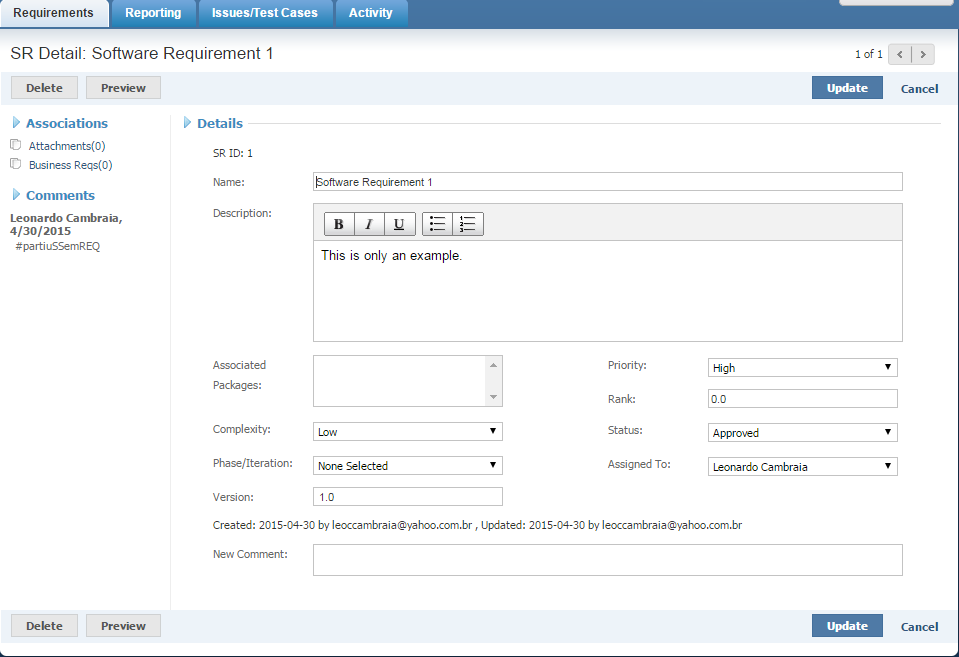
\includegraphics[scale=0.65]{editaveis/figuras/gatherspace_exemplo}
    \caption[Exemplo de um requisito na ferramenta GatherSpace.]
	{Exemplo de um requisito na ferramenta \textit{GatherSpace}.}
    \label{gatherspace_exemplo}
  \end{figure}
  
